\documentclass[../report]{subfiles}
\setcounter{section}{0}
\begin{document}

本章では,食生活を見直し認知症の予防を図るシステム「ふーろぐ」について説明する.
\bunseki{頼亜弥}

\section{ふーろぐの概要}
本グループが開発した「ふーろぐ」の概要を以下で説明する.
まず,撮影者には図\ref{fig:5_box}のボックスを自宅の食卓に置いて頂く.

\begin{figure}[htbp]
    \begin{center}
        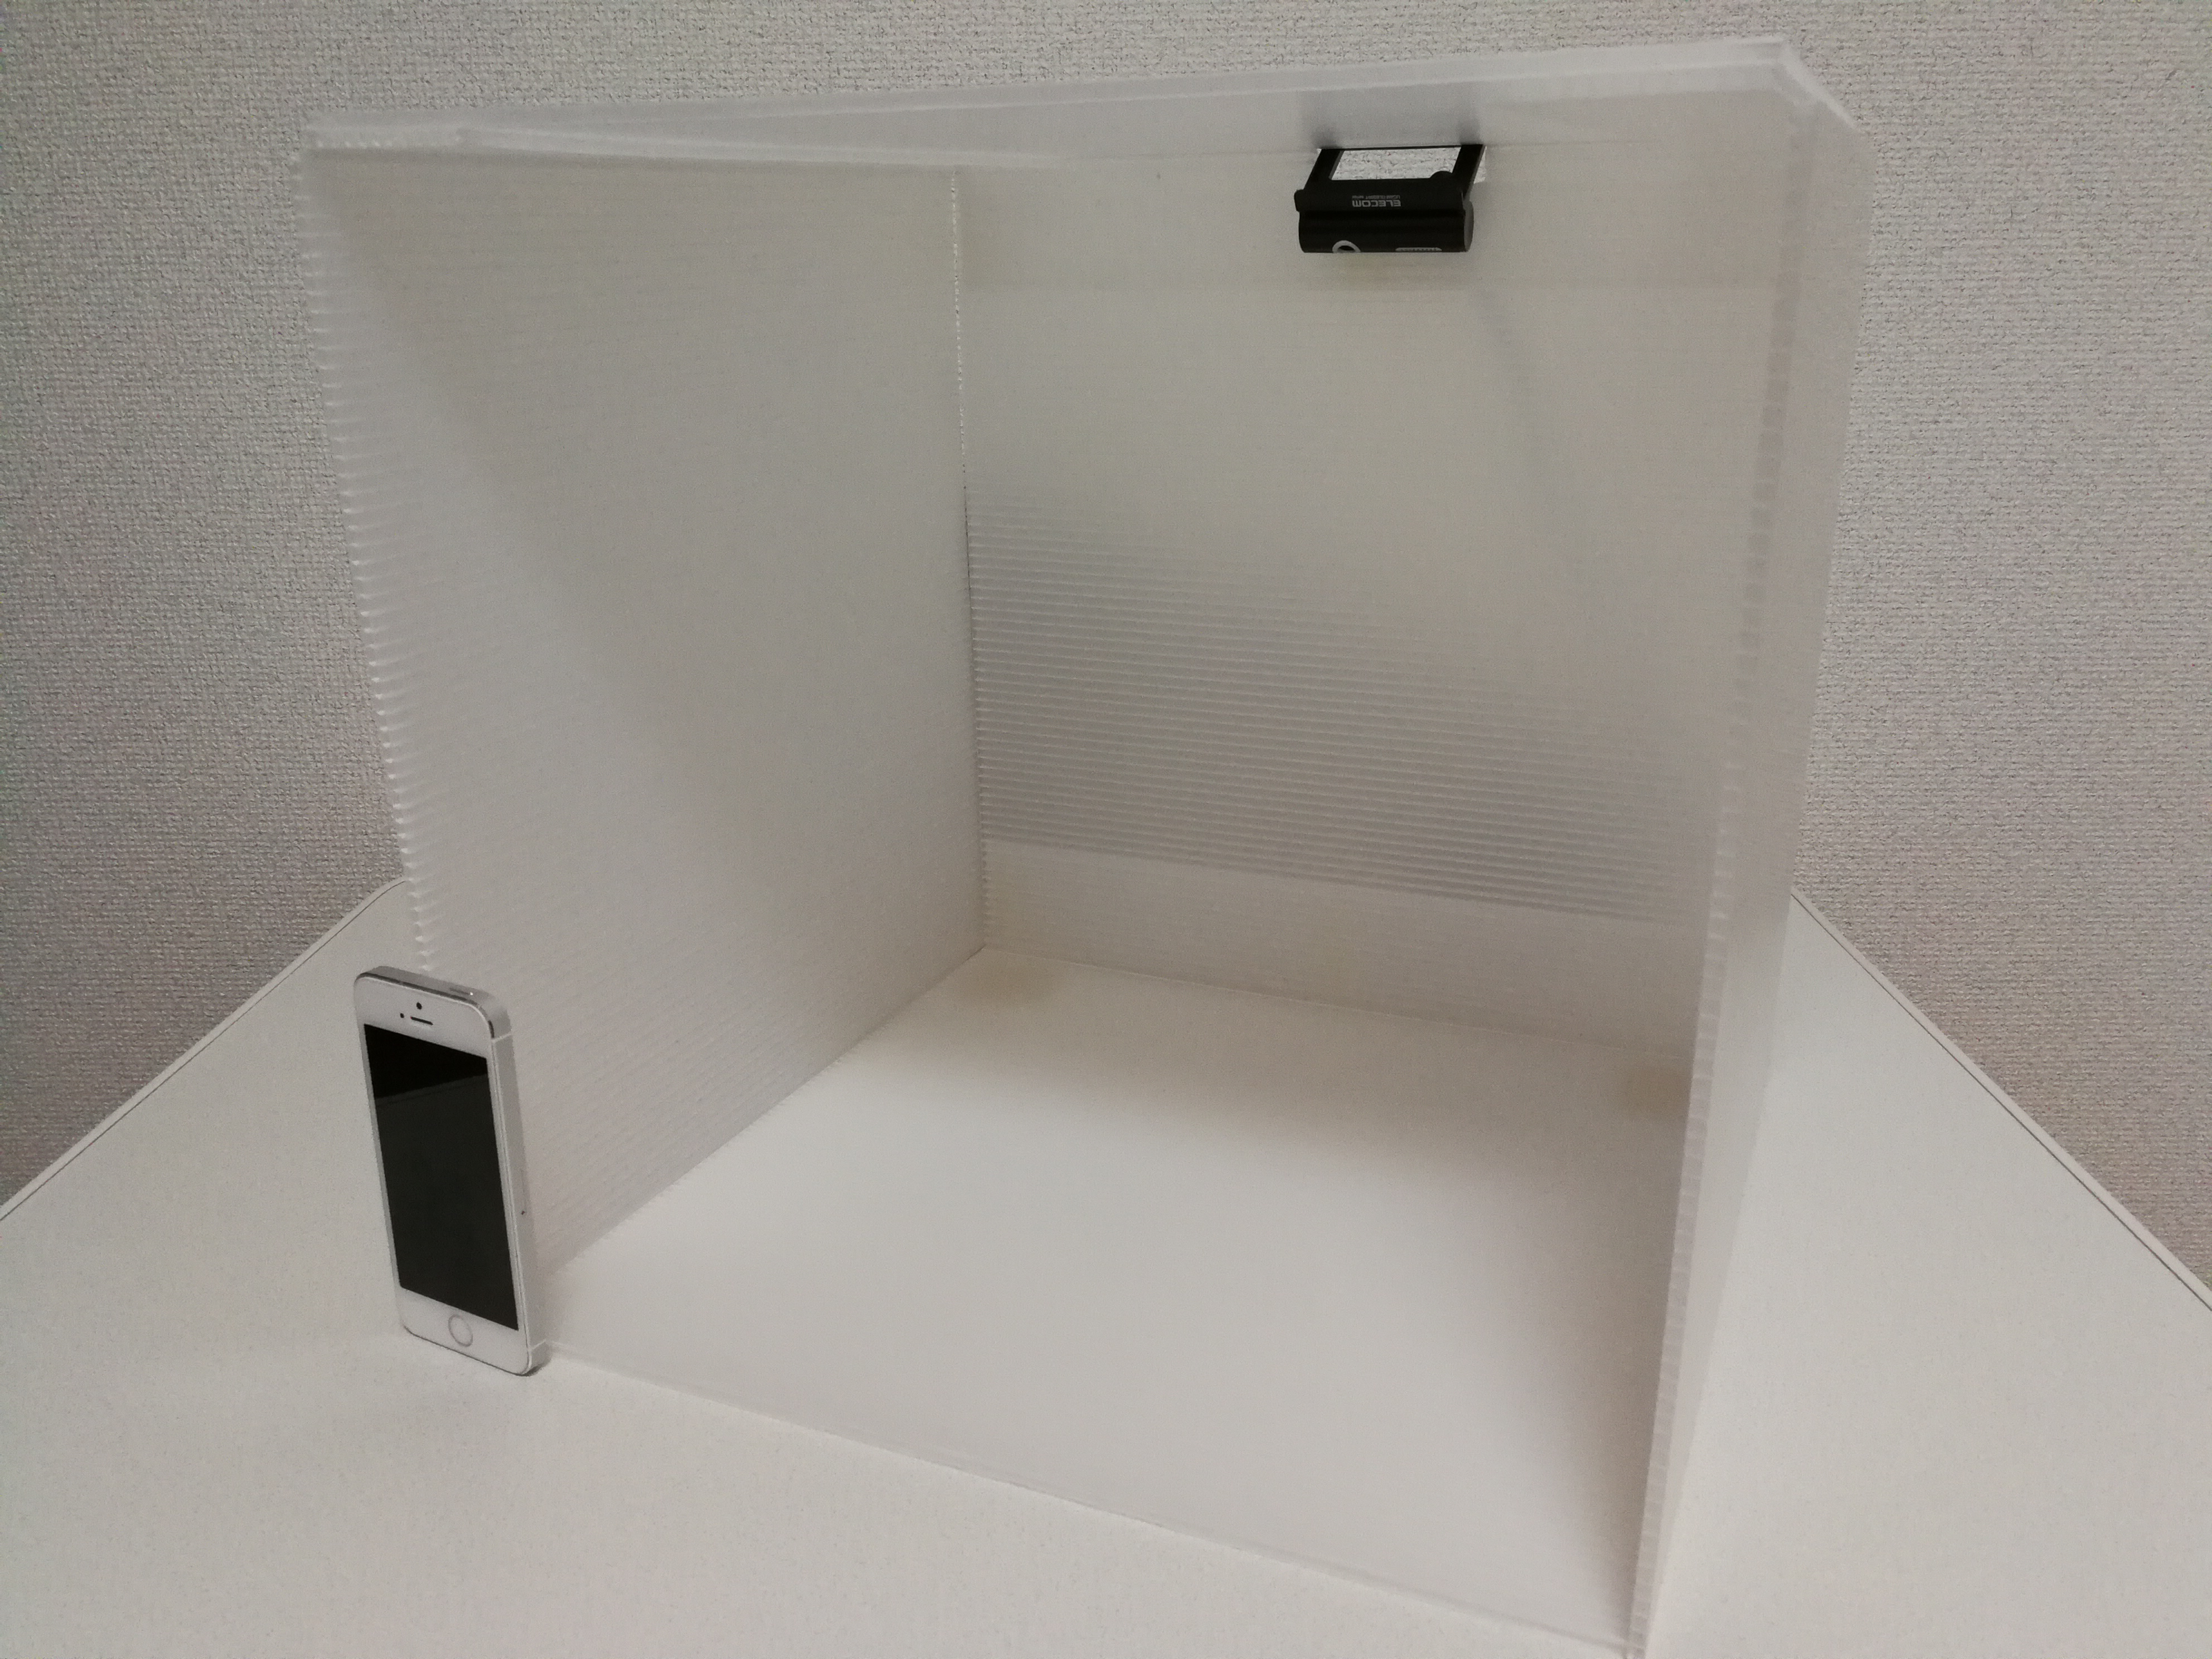
\includegraphics[width=10cm]{imgs/5_box.jpg}
        \caption{撮影用ボックス}
        \label{fig:5_box}
    \end{center}
\end{figure}
\bunseki{頼亜弥}

撮影者がボックスの中に食事を入れると,自動で食事を撮影してくれるという仕組みになっている.
撮影者は,撮った写真をテレビで閲覧できる.
また,撮った写真は家族にも共有して見てもらえる.
医療従事者にも必要に応じて共有できる.

家族・医療従事者側はWebで写真を見れる.
Webでは,撮影者が撮った写真の他に,その写真の食事の栄養素をチャート表示したものを閲覧することもできる.
また,写真に対して撮影者にメッセージを送信できるようになっている.

一方テレビ画面では,今日,昨日,一昨日に撮影した写真を閲覧できる.
撮影した食事の栄養素から,オススメ食事を閲覧することもできる.
また,家族の方から送信されたメッセージも閲覧できる.


\section{ふーろぐのポイント}
本グループが開発した「ふーろぐ」のポイントとして3つ挙げられる.

1つ目は,食生活を簡単に記録できることである.
撮影者は,食事をボックスの中に置くという簡単な動作だけで,食事の写真を撮影できる.
撮影された食事の写真は自動でサーバーに送信され,蓄積されていく仕組みとなっている.
また,撮影者は自宅にあるテレビによって食事の写真を閲覧できる.

2つ目は,離れて暮らす家族とのコミュニケーションを支援できることである.
撮影者は撮影した食事の写真を家族と共有できる.
家族は食事の写真に対し,アドバイスやフィードバックなどを撮影者に向けて送信できる.
撮影者は家族からのメッセージをテレビにて閲覧できる.
撮影者は家族からのメッセージを閲覧することで,食生活に対する意識が変わる.
また,家族とのコミュニケーションのきっかけにもなる.

3つ目は,一人暮らしの高齢者に対する見守り支援になることである.
家族は撮影者の食事の写真を毎日閲覧することで,撮影者の食生活を知れる.
また,撮影者と離れて暮らしていても,食生活を通して撮影者を見守れる.
\bunseki{頼亜弥}


\section{ふーろぐの使い方}
本節では,「ふーろぐ」の使い方を撮影のための「ボックス」,家族などがデータを見たりメッセージを送るための「Web画面」,撮影者がデータを見るための「テレビ画面」に分けて説明する.
補足として,撮影者は一人暮らしの高齢者に当たる.
\bunseki{頼亜弥}

\subsection{撮影用ボックス}
撮影者が日々の食事をボックスの中に置くと,食事の写真が自動で撮影される(図\ref{fig:5_fl}).
撮影者は自宅にあるテレビ画面にて,撮影された写真を閲覧できる.

\begin{figure}[htbp]
    \begin{center}
        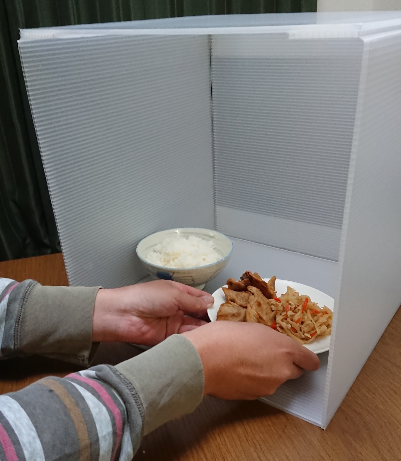
\includegraphics[height=10cm]{imgs/5_fl.png}
        \caption{撮影用ボックスを用いた食事撮影}
        \label{fig:5_fl}
    \end{center}
\end{figure}
\bunseki{頼亜弥}

\subsection{家族他のためのWeb画面}
本節では, 撮影者の家族と医療従事者が閲覧できるWeb画面について説明する.
\bunseki{山根春貴}

\subsubsection{撮影者管理画面}
管理している撮影者を表示する画面である(図\ref{fig:5_dashboard}).
撮影者の名前と撮影者が最後に撮影した時間を表示している.
管理している撮影者をクリックするとカレンダー画面に遷移する.

\begin{figure}[htbp]
    \begin{center}
        \frame{
            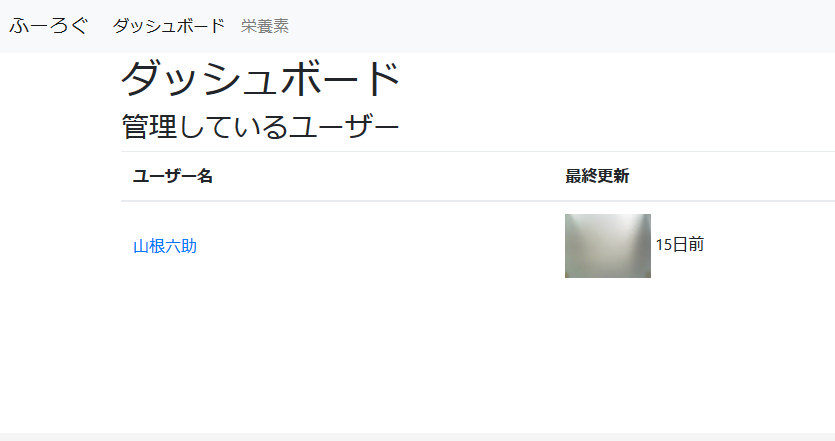
\includegraphics[width=10cm]{imgs/5_dashboard.png}
        }
        \caption{撮影者管理画面}
        \label{fig:5_dashboard}
    \end{center}
\end{figure}
\bunseki{山根春貴}

\subsubsection{カレンダー画面}
対象の撮影者のカレンダー画面である(図\ref{fig:5_calendar-month}).
いつ撮影したか分かりやすくするために,撮影された日は朱色で表示されるようにしている.
カレンダーの日にちをクリックするとデイリー画面に遷移する.

\begin{figure}[htbp]
    \begin{center}
        \frame{
            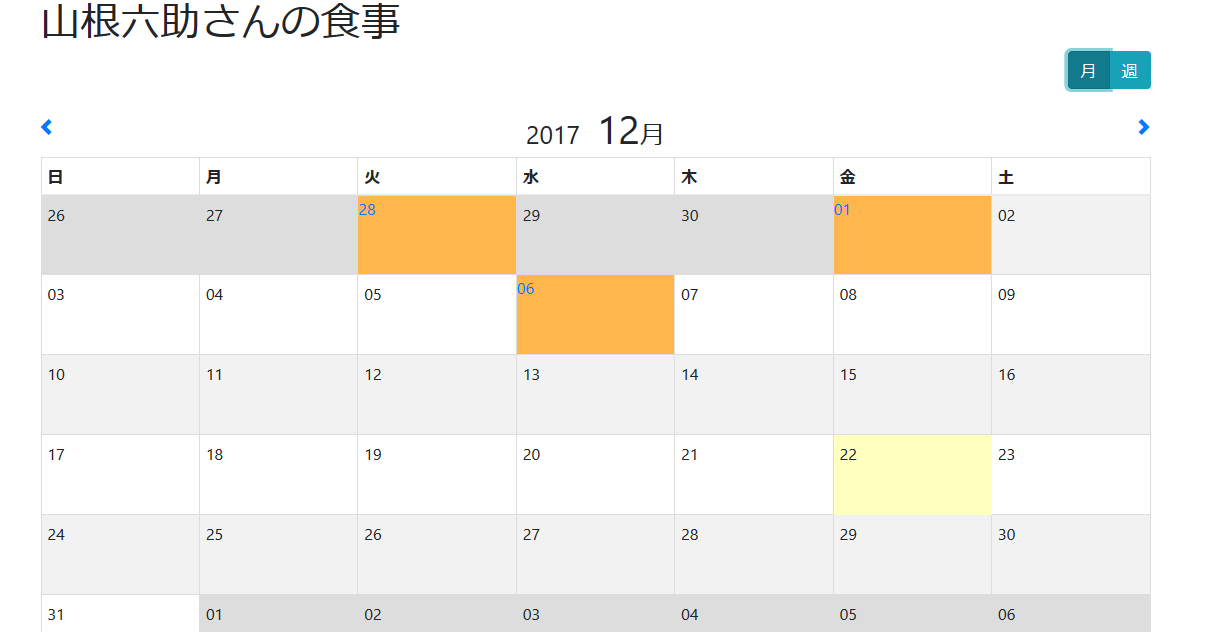
\includegraphics[width=10cm]{imgs/5_month.png}
        }
        \caption{カレンダー画面(月表示)}
        \label{fig:5_calendar-month}
    \end{center}
\end{figure}

また, 「月表示」だけではなく「週表示」に変更することも可能である.
「週表示」の画面では,その日に撮影された写真が表示される(図\ref{fig:5_calendar-week}).

\begin{figure}[htbp]
    \begin{center}
        \frame{
            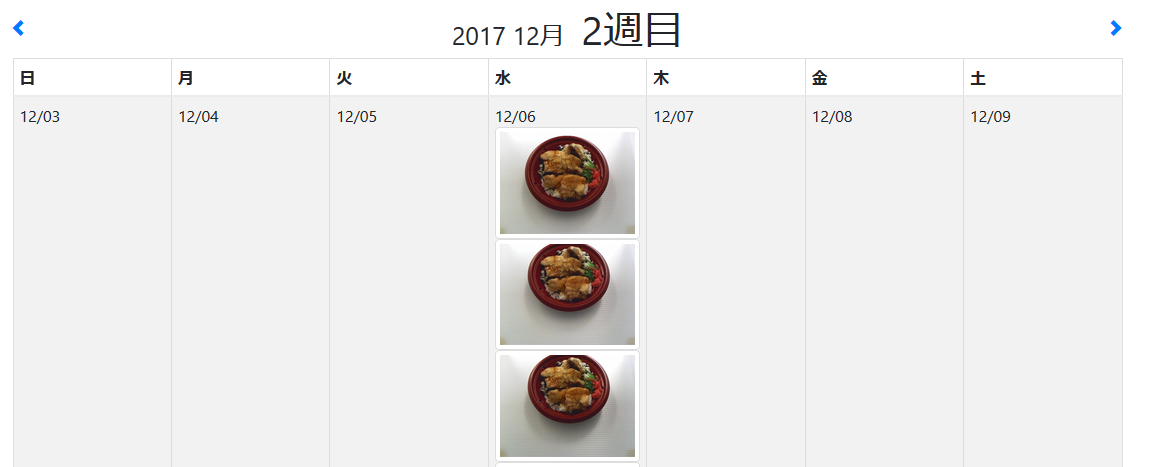
\includegraphics[width=10cm]{imgs/5_week.png}
        }
        \caption{カレンダー画面(週表示)}
        \label{fig:5_calendar-week}
    \end{center}
\end{figure}
\bunseki{山根春貴}

\subsubsection{デイリー画面}
撮影された日の写真と食事名が表示される(図\ref{fig:5_meal}).

\begin{figure}[htbp]
    \begin{center}
        \frame{
            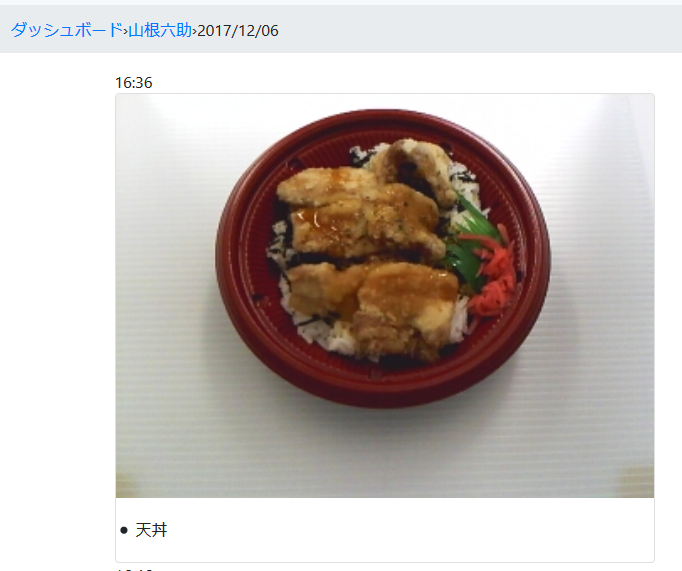
\includegraphics[width=10cm]{imgs/5_day1.png}
        }
        \caption{撮影された食事と食事名}
        \label{fig:5_meal}
    \end{center}
\end{figure}

また, その日の食事が栄養摂取基準に達しているか比較できるレーダーチャートも表示している(図\ref{fig:5_radar}).

\begin{figure}[htbp]
    \begin{center}
        \frame{
            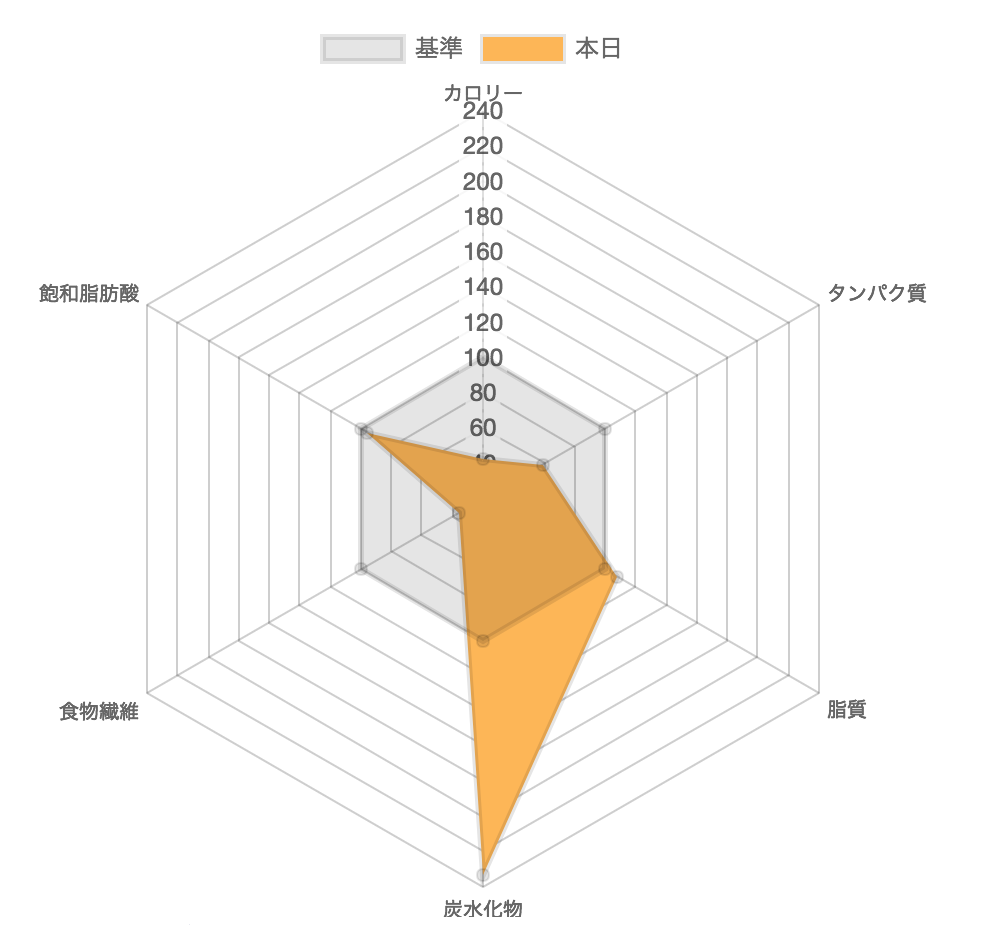
\includegraphics[width=8cm]{imgs/6_radar.png}
        }
        \caption{栄養価のレーダーチャート}
        \label{fig:5_radar}
    \end{center}
\end{figure}

これらの情報から撮影者に対してメッセージ画面を送信することができるようになっている(図\ref{fig:5_message}).
メッセージを送信するとテレビ画面に送信したメッセージが表示される.

\begin{figure}[htbp]
    \begin{center}
        \frame{
            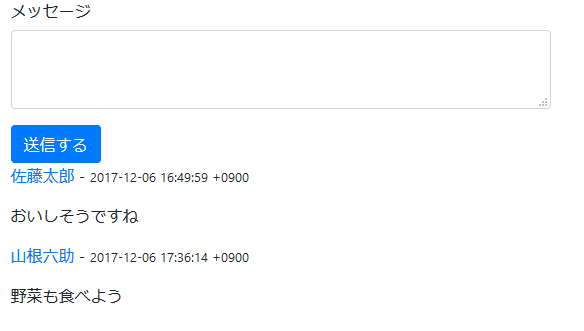
\includegraphics[width=10cm]{imgs/5_day3.png}
        }
        \caption{メッセージ機能}
        \label{fig:5_message}
    \end{center}
\end{figure}
\bunseki{山根春貴}

\subsection{撮影者のためのテレビ画面}
本節では,撮影者が閲覧できるテレビ画面について説明する.
撮影者がICTに不慣れでも扱えるように,一画面に機能を収めている(図\ref{fig:5_tv-all}).

\begin{figure}[htbp]
    \begin{center}
        \frame{
            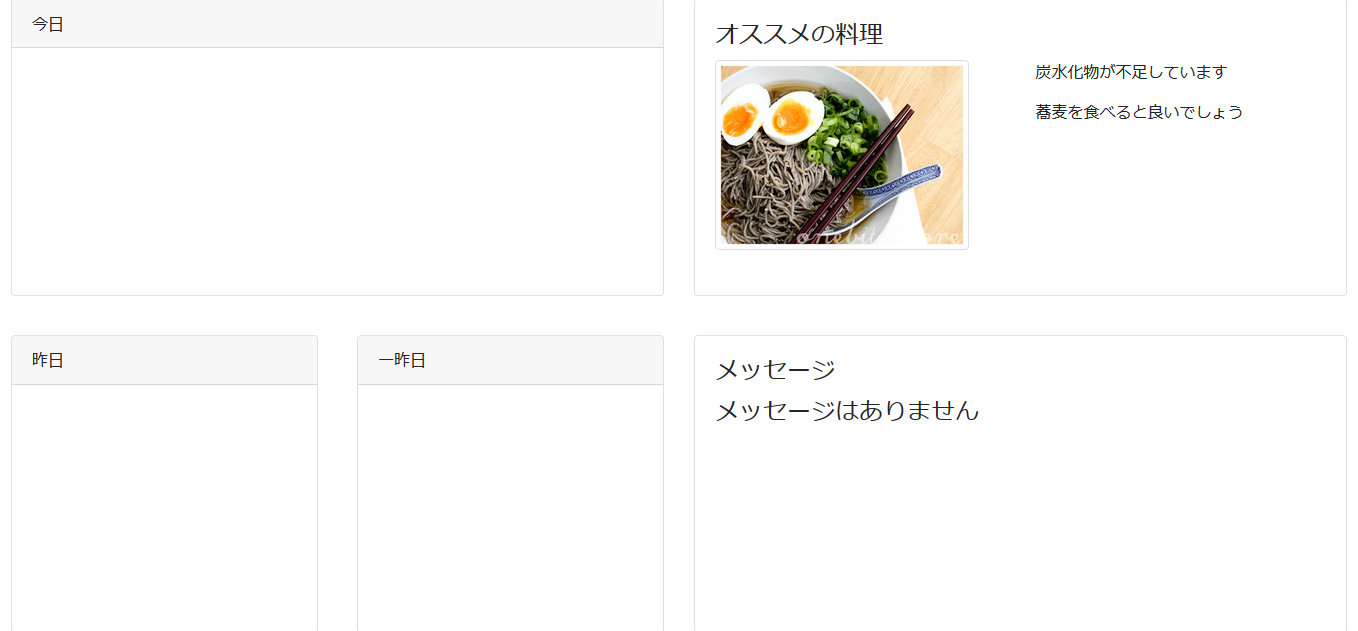
\includegraphics[width=10cm]{imgs/5_tv.png}
        }
        \caption{テレビ画面}
        \label{fig:5_tv-all}
    \end{center}
\end{figure}
\bunseki{山根春貴}

\subsubsection{写真表示機能}
ボックスで自動撮影された写真が表示される.
「一昨日」, 「昨日」, 「今日」の3日分の食事の写真が表示される(図\ref{fig:5_tv-days}).
「今日」の欄には6枚の写真, 「一昨日」と「昨日」の欄には写真が4枚, 一度に見れるようになっている.

\begin{figure}[htbp]
    \begin{center}
        \frame{
            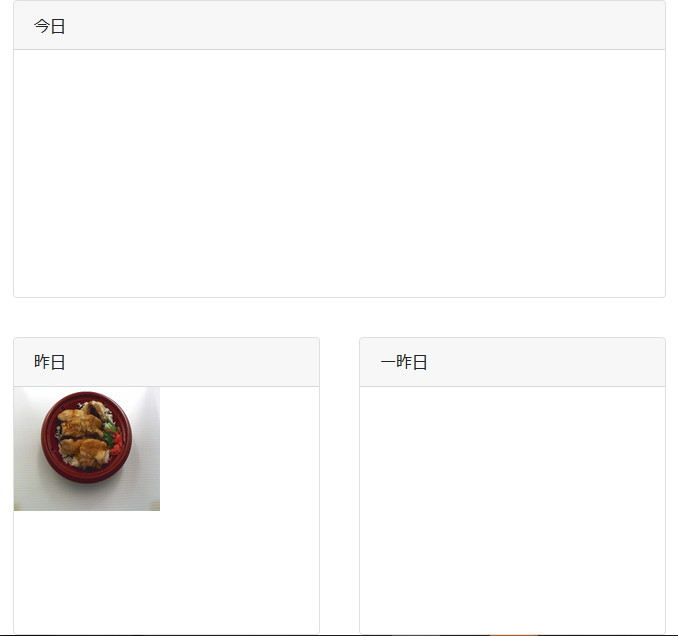
\includegraphics[width=10cm]{imgs/5_tv1.png}
        }
        \caption{写真表示機能}
        \label{fig:5_tv-days}
    \end{center}
\end{figure}
\bunseki{山根春貴}

\subsubsection{オススメの食事提案機能}
ボックスで撮影された写真を1ヶ月分分析し, 平均基準値に満たない栄養素とその栄養素を補えるようなオススメの食事を提案するようになっている(図\ref{fig:5_tv-suggestion}).

\begin{figure}[htbp]
    \begin{center}
        \frame{
            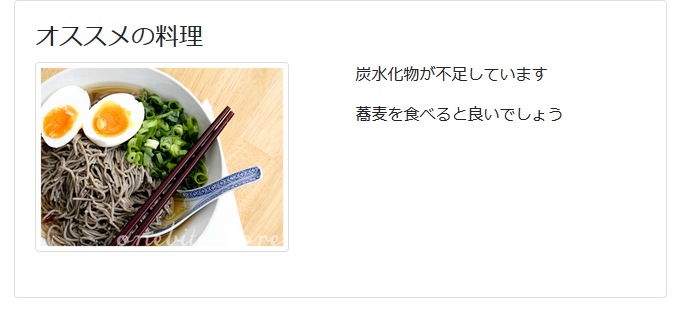
\includegraphics[width=10cm]{imgs/5_tv2.png}
        }
        \caption{オススメ食事提案機能}
        \label{fig:5_tv-suggestion}
    \end{center}
\end{figure}
\bunseki{山根春貴}

\subsubsection{メッセージ機能}
Web画面から送信されたメッセージを確認することができる(図\ref{fig:5_tv-message}).
メッセージが届いた時に誰からメッセージが届いたのか分かるようになっている.

\begin{figure}[htbp]
    \begin{center}
        \frame{
            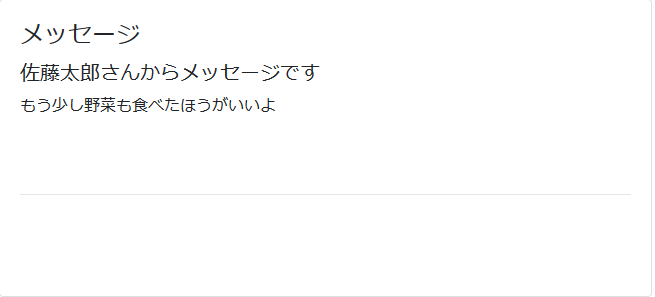
\includegraphics[width=10cm]{imgs/5_message.png}
        }
        \caption{メッセージ機能}
        \label{fig:5_tv-message}
    \end{center}
\end{figure}
\bunseki{山根春貴}
\end{document}
